\documentclass{udpreport}
\usepackage{graphicx}
\usepackage{epstopdf}

% Podemos establecer el logo de alguna entidad o dejar el de la UDP (defecto)
%\setlogo{EITFI}

\title{Métodos Numéricos: Tarea 1}
\author{Ricardo Bravo, Joaquin Cancino, Diego Cardoza, Benjamin Rodriguez}
\email{benjamin.rodriguez@mail.udp.cl \\ joaquin.cancino@mail.udp.cl \\ diego.cardoza@mail.udp.cl \\ ricardo.bravoa@mail.udp.cl}
\date{4 de mayo de 2018}

% Además podemos establecer la facultad y escuela
% los valores por defecto son los siguientes:
\udpschool{Escuela de Informática y Telecomunicaciones}
\udpfaculty{Facultad de Ingeniería}
\udpuniversity{Universidad Diego Portales}

\begin{document}
\maketitle

\tableofcontents
\listoffigures


\chapter{Introducción}
En el presente informe se mostrarán algunos métodos de aproximación a resultados que se tuvieron que programar previamente y probar con funciones dadas por el profesor. 



\section{¿Por qué necesito una sección?}

Cada capítulo a su vez se divide en secciones. A diferencia de un artículo cuyo elemento superior es solo una sección, este documento puede tener capítulos para organizar más información.


\begin{figure}[h]
%Asi agreguen los graficos alksjdha
\centering
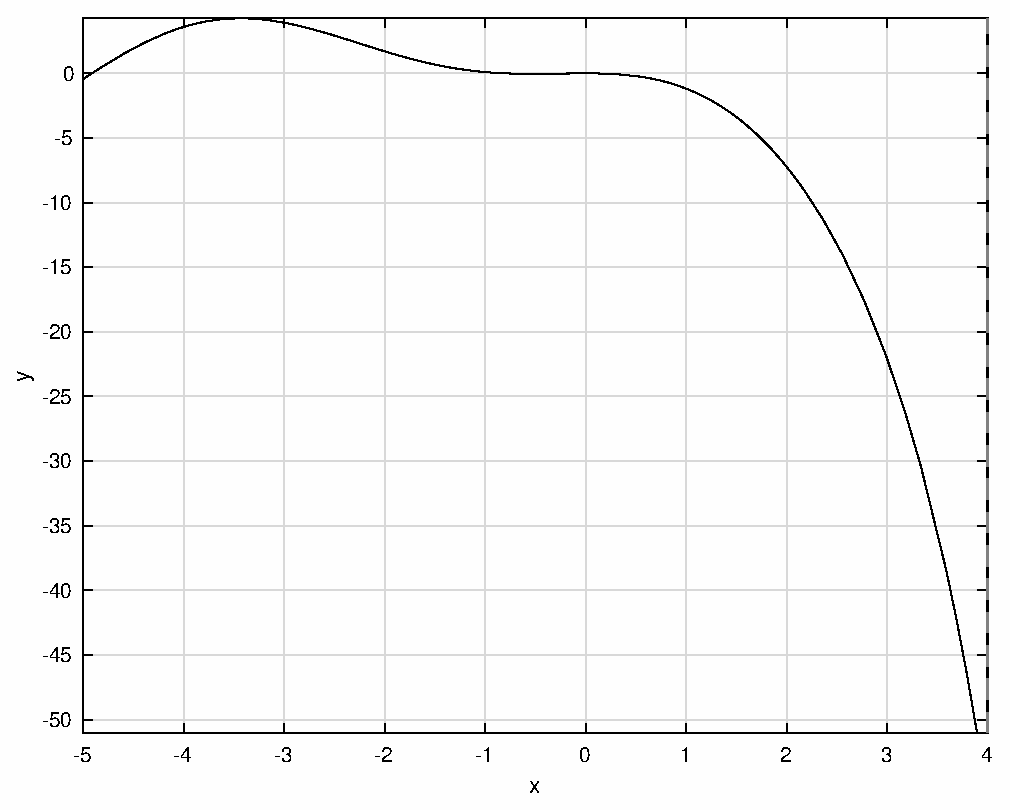
\includegraphics[width=0.5\textwidth]{graficos/PuntoFijo[-5,4].eps}
\caption{Example of a parametric plot ($\sin (x), \cos(x), x$)}
\end{figure}



\chapter{Ejercicio 1}

Se pide programar los métodos de Bisección, Falsa Posición y Secante, y encontrar la raíz aproximada de las siguientes funciones no lineales en los intervalos dados:

\begin{enumarate}  
\item The first item 
\item The second item 
\item The third etc \ldots 
\end{enumarate}

\chapter{Contenido}

Acá otro capítulo.


\end{document}